\section{Lambda}
Ao todo o visitor responsável por pesquisar a adoção de \textit{Lambda} encontrou somente 814 caso de uso. Distribuidos em 354 arquivos o que leva a acreditar que tal característica não esta sendo tão relevante quanto sua espectativa de lançamento. Onde somente 2 casos não estão envolvidos em testes unitátos, os demais 812 estão sendo empregados no desevolvimento de testes unitários conforme exibido pela figura: \ref{fig:AdocaoLambda}. Vale resaltar que somente duas únicas ocorrências de lambda foram encontradas no projeto Jetty versão 9.3.2 nos fontes \textit{PathMap.java} e \textit{RegexSet.java}.\\

\begin{figure}[h]
	\center
	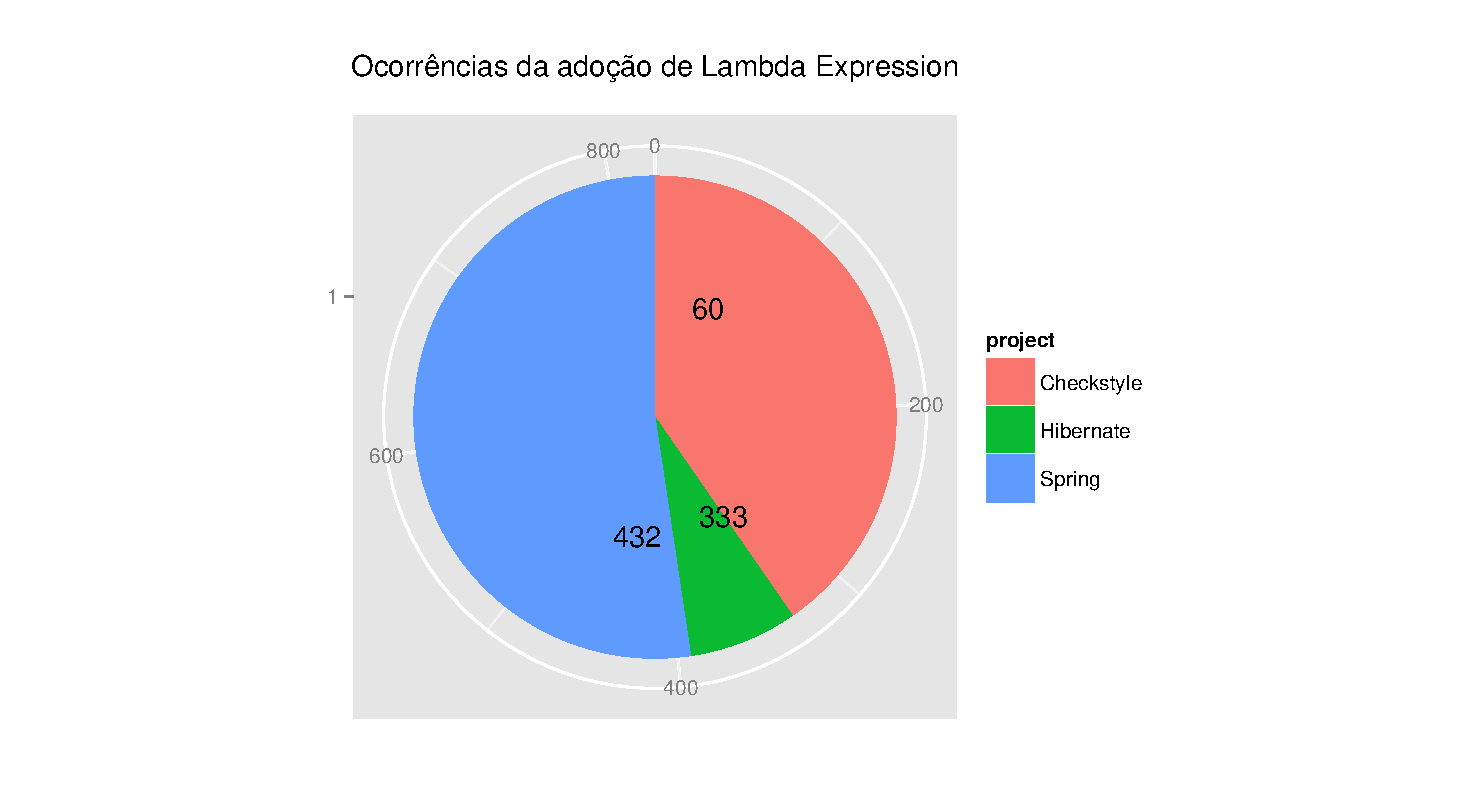
\includegraphics[scale=0.8]{Imagens/AdocaoLambdaTestes}
	\label{fig:AdocaoLambda}
	\caption{Adoção de \textit{Lambda} em testes unitários.}
\end{figure}



\subsection{Oportunidades de Aplicar Lambda}
Entretanto foram encontradas XXXXX oportunidades de converter \textit{For} que iteram \textit{Collections} para \textit{Lambda} através da \textit{Inteface Stream}, totalizando XXX \acs{LOC}. Estas esão dividida confome a figura: \ref{OpportunidadesLambda}.\\
